\paragraph{Breif}
it's a technique we can use when the data distribution is imbalanced, first we define what an "imbalance" is, data is called imbalanced if the output class values aren't evenly represented, for example let's say we study data with output feature having 2 possible values, either 0 or 1, the value 0 happens 80\% of the time while the value 1 is represented by only 20\% of the data, if we start training on this data right away we can expect the trained model to be biased towards the value 0 which appears to be the most common outcome, so even if he value 0 is not ha frequent, the model will assume so because that's what the data say. \newline

the solution for this is to balance the data by removing some instances from the large class(s) until they are close enough to the smaller classes, this way we can decrease the bias of our model towards the large classes, this technique is called \textbf{under sampling}. \newline 

under sampling should solve the problem with bias in the trained model, but at he cost of decreasing the size of the data set when you drop large portion of it, hence decreasing what he model learns, so it can decrease the accuracy as well, if the biggest problem for your model is bias then under sampling can solve it, however if te biggest problem is in learning itself then under sampling shall make it worse.

\paragraph{How we used it in our project}
one of the data sets we worked was imbalanced which made the trained model more biased towards negative emotions (which was more presented in the data set), so we tried to apply under sampling to solve this problem. \newline

\paragraph{results}
unfortunately this made things even worse with our case since the difference between the size of smallest class and other classes was significant(see Figure~\ref{fig:dataset}) so it results in a large decrease in data set size so a large decrease in learning. \newline
\begin{figure}
	\centering
	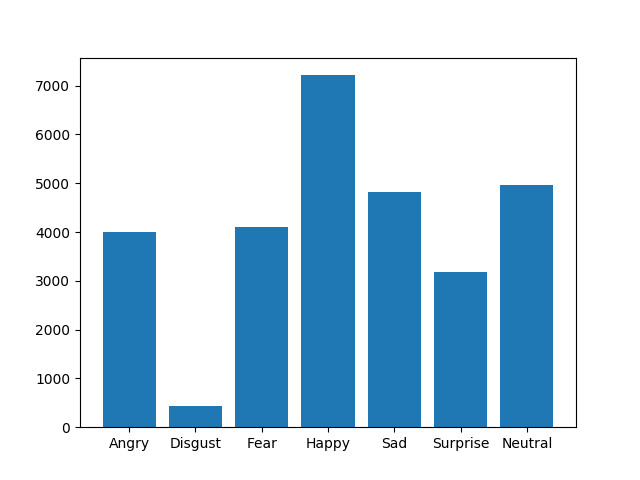
\includegraphics[width=0.75\textwidth]{CH2-Review/sec1_preprocessing/dataset_distribution.png}
	\caption{the unbalanced dataset, classes have large difference in their sizes}
	\label{fig:dataset}
\end{figure}
table \ref{tab:table1} shows the how the prediction accuracy of model changes during training epochs, as the table shows, by more training the training accuracy increases, while testing accuracy actually decreases, so this technique couldn't help solve the overfitting problem we had with the model before it which stopped at about 50\% testing accuracy before overfitting, it even caused a decrease in accuracy, so this technique wasn't a success in his case. 
\begin{table}[h!]
	\centering
	\caption{this table holds the progress of learning for model after under sampling for data set}
	\label{tab:table1}
	\begin{tabular}{c | c | c | c}
		\textbf{Number of Epochs} & \textbf{Training accuracy} & \textbf{Testing accuracy} & \textbf{Error}\\ \hline 
		10 & 39.33 \% & 37.32 \% & 1.69 \\
		20 & 49.08 \% & 36.80 \% & 1.73 \\
		30 & 53.01 \% & 35.64 \% & 1.83 \\
	\end{tabular}
\end{table}